% Created 2024-09-10 Tue 23:52
% Intended LaTeX compiler: pdflatex
\documentclass[12pt]{article}
\usepackage[utf8]{inputenc}
\usepackage[T1]{fontenc}
\usepackage{graphicx}
\usepackage{longtable}
\usepackage{wrapfig}
\usepackage{rotating}
\usepackage[normalem]{ulem}
\usepackage{amsmath}
\usepackage{amssymb}
\usepackage{capt-of}
\usepackage{hyperref}
\usepackage[margin=1in]{geometry} \usepackage{amsmath}
\author{Jason Press}
\date{\today}
\title{Landing a Ball in a Cup Using Projectile Motion}
\hypersetup{
 pdfauthor={Jason Press},
 pdftitle={Landing a Ball in a Cup Using Projectile Motion},
 pdfkeywords={},
 pdfsubject={},
 pdfcreator={Emacs 29.4 (Org mode 9.7.11)}, 
 pdflang={English}}
\begin{document}

\maketitle
\begin{ABSTRACT}


In this lab, we used a ramp and a track to predict the point of impact of a ball that rolled down said ramp and track, and predicted the
\end{ABSTRACT}
\section{Introduction}
\label{sec:org393cc0a}

The aim of this lab was to have a ball roll off a track and into a cup on the ground. To get the ball rolling, it started from the top of a ramp, rolled down the ramp when released to gather velocity in the \(x\) direction, ran along a track with a pair of photogates to measure the speed along with ensuring the \(y\) component of the velocity was zero, and then rolled off the end of the track to land in a cup on the ground. To know where to place the cup, we calculated the speed of the ball by repeatedly releasing it from the ramp and having it run through a pair of photogates to measure the time. Knowing the time it took for the ball to travel between the photogates \(t_1\), and by measuring the distance between the photogates \(d\), we calculated the average velocity in the \(x\) direction using \(\bar{v}_{x0} = \frac{d}{\bar{t}_{1}}\) using the average time measurement of ten trial runs.

In order to know where to place the cup, we needed to obtain the time in free fall. To get the time of the ball in free fall, we used the kinematic equation for constant acceleration in the \(y\) direction and solved for the free fall time \(t_{2}\):


\begin{align}
y_{f} = y_{0} + v_{0y}t_{2} + \frac{1}{2} a_{y}t_{2}^{2} \\
\text{Assume } y_{f} = 0\text{, }y_{0} = h\text{, } v_{0y} = 0\text{, and } a_{y} = -g \\
0 = h - \frac{1}{2} g t_{2}^{2}
\end{align}

This ultimately yields an equation for solving for \(t_2\) using only known quantities:

\begin{align}
        t_{2} = \sqrt{\frac{2h}{g}}
\end{align}

Using a known value for \(t_2\), we can substitute into the distance equation for \(\Delta x\) assuming the ball starts falling at \(x_0 = 0\) with no \(x\) acceleration:

\begin{equation} \label{xf-eqn}
x_{f} = \frac{d}{t_{1}}\sqrt{\frac{2h}{g}}
\end{equation}

Then, we placed a cup \(x_f\) meters away from the table, released the ball from the top of the ramp in the same manner as in the trial runs (the ones to obtain the \(x\) component of the ball's velocity), and witnessed the ball land perfectly in the cup.
\section{Methods}
\label{sec:orgaa4fbb6}

The main source of uncertainty in this lab was the initial release of the ball onto the ramp to gain acceleration. To minimize the error, we pushed the ball up the back face of the ramp until it started falling on the main side of the ramp. We did this as to impart minimal initial velocity on the ball, so the ball would accelerate for the same amount of time and reach the same end speed.

We performed ten trial runs to obtain an average velocity in the \(x\) direction. We used ten runs since there was a slight run to run variation, and obtaining the average over ten runs allowed for an accurate prediction of \(v_{x0}\) for the actual run. For the trial runs, we stopped the ball from falling onto the ground by placing a member at the end of the track to collect the ball after it passed through the photogates, allowing us to get a measurement of \(t_1\), but without allowing the ball to fall to the ground.

To measure the distance at which to place the cup on the ground, we positioned the end of the track to be at the edge of the table. We used one meterstick to measure the height from the ground to the top of the track to obtain the height of the track. Additionally, we measured the height of the cup, since we want the ball to fall into the mouth of the cup rather than the base of the cup (if we did not account for the height of the cup, the ball would hit the side of the cup instead of going into the cup). While we had the meterstick lined up with the edge of the table, we used a second meterstick positioned on the ground to measure the \(x\) distance from the start of the track, placing the cup at the calculated distance and in line with the line the ball would travel through.

With the cup positioned at the predicted point of impact, we released the ball in the same manner as the trial runs. With the measurements done properly, we released the ball, it rolled down the track, off the edge, and passed through the center of the cup, landing in the cup.

Here is the experiment setup:

\begin{center}
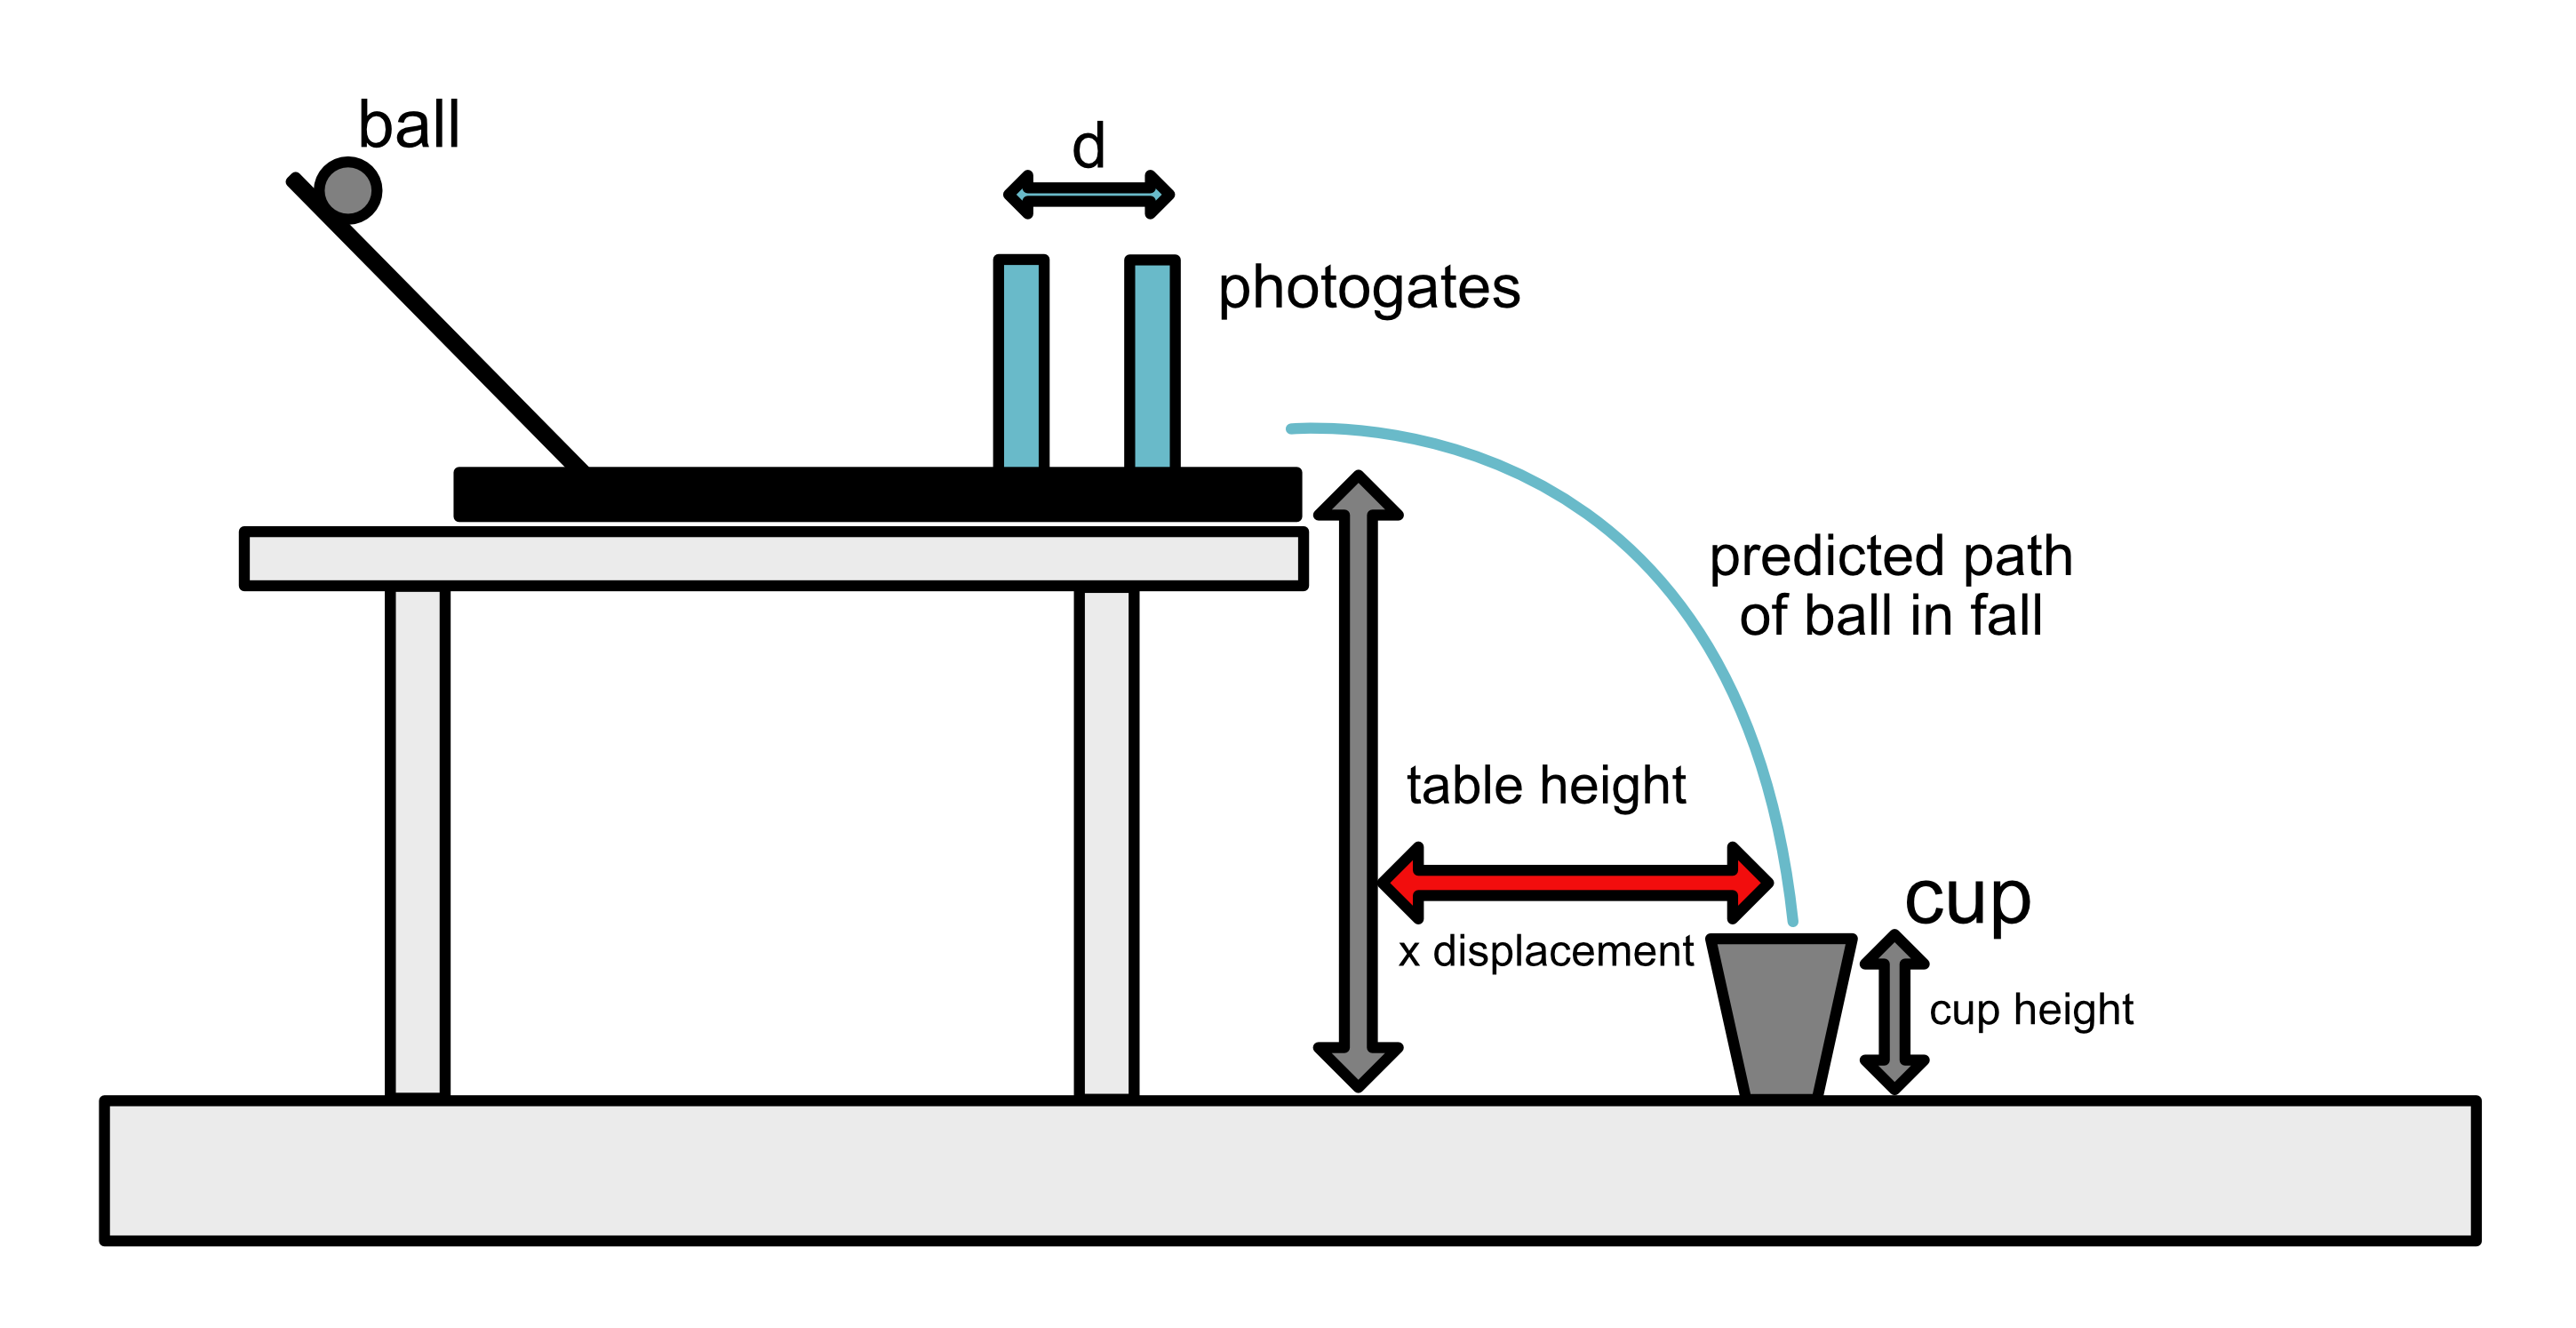
\includegraphics[width=6in]{./projectilesetup.png}
\captionof{figure}{\label{fig:track}Track setup}
\end{center}
\section{Results}
\label{sec:orgefb2762}

For all calculations, we assume \(g\) to be 9.81\(\frac{\text{m}}{\text{s}^{2}}\).

Here is the results of our trial runs:
\begin{center}
\captionof{table}{Trial run results}
\begin{tabular}{r|r}
\hline
Run & Time (s)\\
\hline
1 & 0.0366\\
2 & 0.0359\\
3 & 0.0375\\
4 & 0.0392\\
5 & 0.0367\\
6 & 0.0378\\
7 & 0.0391\\
8 & 0.0369\\
9 & 0.0387\\
10 & 0.0362\\
\hline
Average (\(\bar{t}_{1}\)) & 0.0375\\
Standard error & 0.000380\\
\end{tabular}
\end{center}

Here is the prediction of \(x_f\) using the other measurements:

\begin{center}
\captionof{table}{\label{table:results}Predicted values}
\begin{tabular}{l|l}
\hline
Quantity & Amount\\
\hline
\(d\) & 0.075m\\
\(\bar{t}_{1}\) & 0.0375s\\
Cup height & 0.124m\\
Table height & 0.936m\\
\(h\) & 0.812m\\
\(x_f\) & 0.814m\\
Error & 0.0263m\\
\end{tabular}
\end{center}

When we released the ball, it rolled down the ramp, off the track, and landed in the cup.
\section{Discussion}
\label{sec:org7d1481f}

Our ball landed in the cup. The small amount of error reflects that fact.

The amount of error for the time measurement is small because we used a photogate. The error for time is as follows:

\begin{center}
\captionof{table}{\label{table:photoerror}Photogate error}
\begin{tabular}{l|l}
\hline
Error source & Value\\
\hline
\(\sigma_{t,stat}\) & 0.000380s\\
\(\sigma_{t,res}\) & 0.00005s\\
\(\sigma_{t,sys}\) & 0.001s\\
\hline
\(\sigma_t\) & 0.00107s\\
\end{tabular}
\end{center}

We used the standard error of the trial runs for the time measurement for the statistical error for time, since there was a small amount of variability between trial runs. The resolution error of the photogate is half of the resolution of the photogate (the resolution was 0.0001s). The systematic error is half of the resolution of the measuring tape for each gate's placement. We account for this error with \(\sigma_d\).

We used the same measuring device for both \(d\) and \(h\), used in the same manner. Thus, they have the same error values, i.e. \(\sigma_h = \sigma_d\). The error for the meterstick is as follows:

\begin{center}
\captionof{table}{\label{table:metererror}Meterstick error}
\begin{tabular}{l|l}
\hline
Error source & Value\\
\hline
\(\sigma_{h,stat}\) & 0m\\
\(\sigma_{h,res}\) & 0.0005m\\
\(\sigma_{h,sys}\) & 0.001\\
\hline
\(\sigma_h\) & 0.0012m\\
\end{tabular}
\end{center}

We assumed that the statistical error for the meterstick is zero, since repeated measurements yield the same result. Each group member independently verified each measurement to minimize statistical error. The resolution error of the meterstick is half the resolution of the meterstick (the resolution was 0.0005m). We determined the systematic error of the meterstick to be 0.001m, since there were two measurements in the photogate, each one being within half of the resolution of the meterstick, and measuring the proper height of the track was hard because we held the meterstick at a close but not perfect \(90^{\circ}\) since we did not have a speed square to ensure a \(90^{\circ}\) angle between the meterstick and ground.

One major source of error not accounted for properly in the error calculation is the error of placing the cup in the correct spot. We calculated the error for the experiment using the following equation:

\begin{equation} \label{eqn:std-err}
\sigma_{x}^{2} &= \left( \frac{1}{t_{1}}\sqrt{\frac{2h}{g}} \right)^{2} \sigma_{d}^{2} + \left( - \frac{d}{t_{1}^{2}}\sqrt{\frac{2h}{g}} \right) ^{2} \sigma_{t}^{2} + \left( \frac{d}{2t_{1}} \sqrt{\frac{2}{gh}} \right)^{2} \sigma_{h}^{2}
\end{equation}

That source of error is not accounted for in any of the aforementioned measurements: \(\sigma_h\) is the error in the height measurement, and \(\sigma_d\) is the error in the photogate distance measurement. In other words, the error of placing the cup at the right place is not represented in Equation \ref{eqn:std-err}. We took steps in the procedure to minimize this error, like using a second meterstick to align \(x_0\), but we did not assign a numerical value to the error.

However, in the end, we managed to put a ball in a cup.
\section{Sample Calculations}
\label{sec:orgd4621e5}

We performed all calculations in a spreadsheet. We recorded the ten trial runs from \texttt{A4:A13}.

To calculate the average of the ten runs, we used \texttt{AVERAGE(A4:A13)}. To calculate the height the ball would fall, we subtracted the table height from the cup height. To calculate the predicted \(x_f\), we did \texttt{A2/A15*SQRT(2*D2/9.81)}.

To calculate \(\sigma_{t,stat}\), we used \texttt{STDEV(A4:A13)/sqrt(10)}. To calculate \(\sigma_t\) and \(\sigma_h\), we took the square root of the sum of squares of the related error values. For example, we calculated \(\sigma_t\) with \texttt{=SQRT(B17\textasciicircum{}2+B18\textasciicircum{}2+B19\textasciicircum{}2)}. Finally, we used the spreadsheet version of Equation \ref{eqn:std-err} to calculate the error, which is as follows:
\begin{verbatim}
SQRT((1/A15*SQRT(2*D2/9.81))^2*H20^2+
    (-A2/A15^2*SQRT(2*D2/9.81))^2*B20^2+
    (A2/2*A15*SQRT(2/9.81*D2))^2*E20^2)
\end{verbatim}

\begin{center}
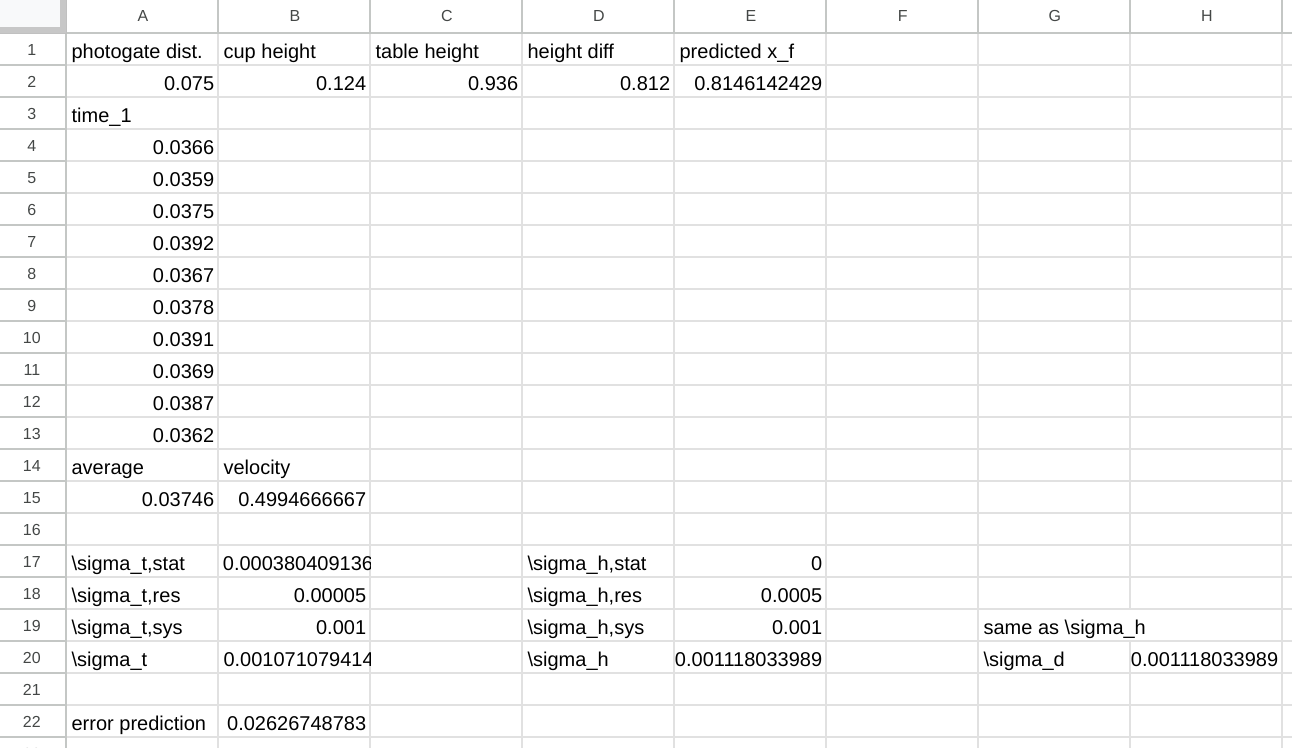
\includegraphics[width=6.5in]{./spreadsheet.png}
\captionof{figure}{\label{fig:spreadsheet}Spreadsheet}
\end{center}
\end{document}
